\documentclass{article}

\usepackage{tikz}
\usetikzlibrary{positioning} % for "right=of" etc.

% Define a custom environment "tikzfigure" that wraps figure + centering
\newenvironment{tikzfigure}[1][htbp]
{%
  \begin{figure}[#1]%
  \centering
}
{%
  \end{figure}%
}

\begin{document}

\begin{tikzfigure}
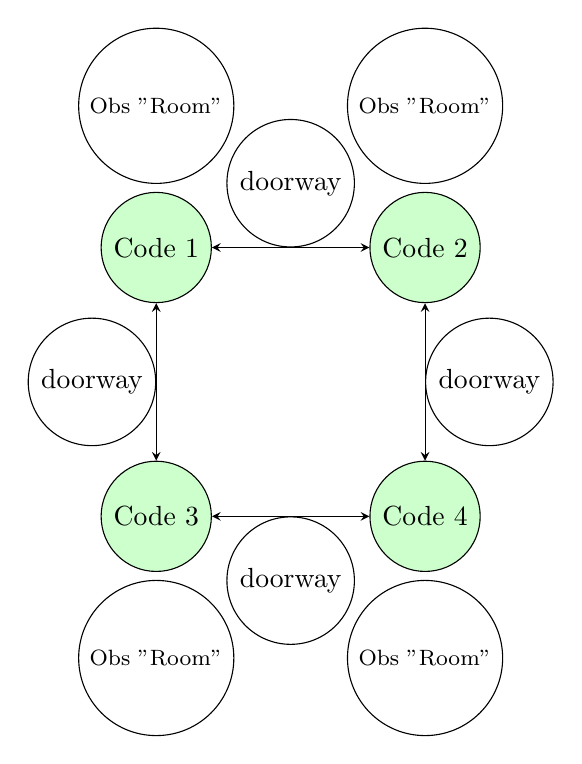
\begin{tikzpicture}[node distance=2cm, >=stealth, every node/.style={draw, circle, minimum size=1cm}]
  % Nodes
  \node[fill=green!20] (s1) {Code 1};
  \node[fill=green!20, right=2cm of s1] (s2) {Code 2};
  \node[fill=green!20, below=2cm of s1] (s3) {Code 3};
  \node[fill=green!20, below=2cm of s2] (s4) {Code 4};

  % Observations label (same for all)
  \node[above=0.1cm of s1, font=\footnotesize] {Obs "Room"};
  \node[above=0.1cm of s2, font=\footnotesize] {Obs "Room"};
  \node[below=0.1cm of s3, font=\footnotesize] {Obs "Room"};
  \node[below=0.1cm of s4, font=\footnotesize] {Obs "Room"};

  % Bidirectional transitions
  \draw[<->] (s1) -- node[above]{doorway} (s2);
  \draw[<->] (s1) -- node[left]{doorway} (s3);
  \draw[<->] (s4) -- node[below]{doorway} (s3);
  \draw[<->] (s4) -- node[right]{doorway} (s2);
\end{tikzpicture}
\caption{A simple four-code map showing aliased observations and doorways.}
\label{fig:code_map}
\end{tikzfigure}

\end{document}
